\subsection{Angriffseinheiten}\label{sec:attack}

\newlength{\bodywidth}
\setlength{\bodywidth}{\textwidth}
\addtolength{\bodywidth}{-12pt}

\begin{description}
  \item[Truppen]
    kosten relativ wenig, lassen sich jedoch nicht weiter kontrollieren.
    Sie sind einer Welle zugeordnet und spawnen gemeinsam mit den anderen
    Truppen dieser Welle. Sie verfolgen das Ziel, auf dem kürzesten Weg das
    gegenerischen Lager zu erreichen um dort Schaden zu verursachen.


  \item[Helden] kosten mehr als Truppen, diese Einheiten lassen sich jedoch vom
    Spieler kontrollieren und so strategisch einsetzen und außerhalb der
    Reichweite von Verteidigungsgebäuden positionieren; zusätzlich besitzen sie
    Fähigkeiten, die der Spieler einsetzen kann. Es ist nicht möglich, mehr als
    einen Helden einer Art zum gleichen Zeitpunkt am Leben zu haben. Helden
    sind keiner Welle zugeordnet, sie spawnen direkt beim Kauf.

\end{description}

Tabelle~\ref{tab:attack-unit-props} beschreibt die Eigenschaften die
Angriffseinheiten haben, in Tabelle~\ref{tab:attack-units} sind alle Truppen
mit ihren Eigenschaften aufgelistet und Tabelle~\ref{tab:attack-heroes} enthält
alle Helden.

\begingroup
  \small
  \begin{longtabu}{rlX}
    \rowfont{\normalsize}
    \caption{Eigenschaften von Angriffseinheiten\label{tab:attack-unit-props}}\\

    \midrule[\heavyrulewidth]\rowfont{\itshape}
    & Eigenschaft & Beschreibung \\
    \midrule

    K  & Kosten
       & Die Menge an Bitcoin die aufgewendet werden muss, um eine dieser
         Einheiten zu kaufen (\refid{A:buy-attack}). \\
    LP & Lebenspunkte
       & Die Zahl der Lebenspunkte einer Einheit: Angriffe von
         Verteidigungstürmen ziehen Lebenspunkte von diesem Wert ab; fällt er
         unter Null, so stirbt diese Einheit (\refid{A:die}). \\
    AS & Angriffsstärke
       & Schaden, den diese Einheit am gegenerischen Lager verursacht, wenn sie
         dieses erreicht (\refid{A:damage-base}). \\
    GS & Geschwindigkeit
       & Distanz, die pro Zeiteinheit zurückgelegt werden kann. \\

    \bottomrule
  \end{longtabu}
  \todo[inline, caption = {Größe und Kollision}]{%
    Größe und Kollision evtl. in die Tabelle aufnehmen, aber was sagt die Größe
    genau aus? Diese ist doch nur interessant, wenn die Einheit kollidiert?}
\endgroup

\pagebreak
\begingroup
  \small
  \begin{longtabu}{XXXX}
    \rowfont{\normalsize}
    \caption{Truppen und ihre Werte\label{tab:attack-units}}
    \\\midrule[\heavyrulewidth]\endfirsthead

    \rowfont{\normalsize}
    \caption[]{Truppen und ihre Werte (fortges.)}
    \\\midrule[\heavyrulewidth]\endhead

    \multicolumn{4}{r}{\itshape fortges. auf der nächsten Seite}
    \\\endfoot

    \endlastfoot

    \multicolumn{4}{c}{\bfseries Bug} \\*
    K: 2 & LP: 4 & AS: 1 & GS: 7 \\\midrule
    \multicolumn{4}{p{\bodywidth}}{%
      \begin{minipage}{0.85\linewidth}
        Eine schnelle Sprintereinheit ohne viele Lebenspunkte, die alleine
        nicht besonders viel Schaden verursacht, aber in großer Masse gekauft
        werden kann, da sie nicht viel kostet.
      \end{minipage}\hfill\parbox{0.15\linewidth}{%
        \hfill
\includegraphics[scale=0.9]{angriff/bug.png}\hfill\null}}
    \\\bottomrule

    \multicolumn{4}{c}{\bfseries Virus} \\*
    K: 3 & LP: 10 & AS: 2 & GS: 5 \\\midrule
    \multicolumn{4}{p{\bodywidth}}{%
      \begin{minipage}{0.85\linewidth}
         Durchschnittliche Einheit, die etwas mehr kostet als ein \emph{Bug,}
         etwas langsamer ist, aber mehr LP hat und mehr Schaden verursacht.
      \end{minipage}\hfill\parbox{0.15\linewidth}{%
        \hfill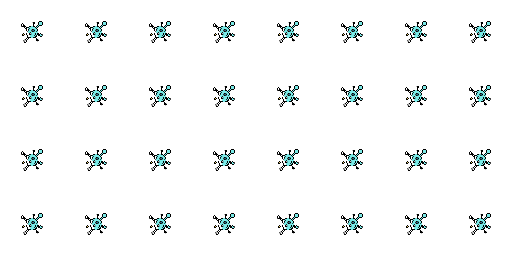
\includegraphics[scale=0.7]{angriff/virus.png}\hfill\null}}
    \\\bottomrule

    \multicolumn{4}{c}{\bfseries Trojaner} \\*
    K: 20 & LP: 30 & AS: 6 & GS: 3 \\\midrule
    \multicolumn{4}{p{\bodywidth}}{%
      \begin{minipage}{0.85\linewidth}
         Stirbt diese Einheit, werden an der Stelle ihres Todes fünf \emph{Bugs}
         gespawnt (\refid{A:spawn-children}). Ein Trojaner ist zwar relativ
         langsam und kostet mehr als \emph{Viren,} hat dafür aber mehr LP und
         mehr AS.
      \end{minipage}\hfill\parbox{0.15\linewidth}{%
        \hfill
\includegraphics[scale=0.6]{angriff/trojan.png}\hfill\null}}
    \\\bottomrule

    \multicolumn{4}{c}{\bfseries Nokia} \\*
    K: 30 & LP: 100 & AS: 15 & GS: 2 \\\midrule
    \multicolumn{4}{p{\bodywidth}}{%
      \begin{minipage}{0.85\linewidth}
         Diese Einheit ist bei gleichen Kosten zwar langsamer als ein
         \emph{Trojaner,} dafür aber hat sie mehr LP und AS.
      \end{minipage}\hfill\parbox{0.15\linewidth}{%
        \hfill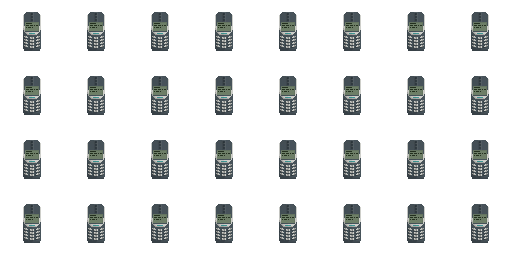
\includegraphics[scale=0.6]{angriff/nokia.png}\hfill\null}}
    \\\bottomrule

    \multicolumn{4}{c}{\bfseries Thunderbird} \\*
    K: 15 & LP: 15 & AS: 3 & GS: 3 \\\midrule
    \multicolumn{4}{p{\bodywidth}}{%
      \begin{minipage}{0.85\linewidth}
         Diese Einheit fliegt, daher muss sie nicht den
         Weg um Mauern und Türme herumfinden, sondern kann einfach auf
         Luftlinie darüber hinwegfliegen.

         Von der Geschwindigkeit ist diese Einheit mit \emph{Trojaner}
         vergleichbar, sie ist zwar etwas günstiger, und hat nur halb so viele LP.
      \end{minipage}\hfill\parbox{0.15\linewidth}{%
        \hfill
\includegraphics[scale=0.6]{angriff/thunderbird.png}\hfill\null}}
    \\\bottomrule
  \end{longtabu}
\endgroup


\begingroup
  \small
  \begin{longtabu}{XXXX}
    \rowfont{\normalsize}
    \caption{Helden und ihre Werte\label{tab:attack-heroes}}
    \\\midrule[\heavyrulewidth]\endfirsthead

    \rowfont{\normalsize}
    \caption[]{Helden und ihre Werte (fortges.)}
    \\\midrule[\heavyrulewidth]\endhead

    \multicolumn{4}{r}{\itshape fortges. auf der nächsten Seite}
    \\\endfoot

    \endlastfoot

    \multicolumn{4}{c}{\bfseries Settings} \\*
    K: 50 & LP: 25 & AS: 0 & GS: 4 \\\midrule
    \multicolumn{4}{p{\bodywidth}}{%
      \begin{minipage}{0.85\linewidth}
        Diese Einheit heilt andere Truppen, hat dafür jedoch eher wenig LP;
        dies ist die langsamste Heldeneinheit, sie verursacht am gegenerischen
        Lager keinen Schaden.

        \emph{Fähigkeit:} Heilt alle zwei Sekunden, Truppen im Radius von 1
        Kachel um 2 LP. Dies ist eine passive Fähigkeit.
      \end{minipage}\hfill\parbox{0.15\linewidth}{%
        \hfill
\includegraphics[scale=0.6]{angriff/settings.png}\hfill\null}}
    \\\bottomrule\pagebreak

    \multicolumn{4}{c}{\bfseries Firefox} \\*
    K: 50 & LP: 30 & AS: 10 & GS: 6 \\\midrule
    \multicolumn{4}{p{\bodywidth}}{%
      \begin{minipage}{0.85\linewidth}
        Dieser Held ist eine starke Angriffseinheiten, die mit ihrer Fähigkeit
        leichter zwischen den Verteidigungsgebäuden hindurchkommt. Der
        \emph{Firefox} ist relativ schnell, hat durchschnittliche LP und
        relativ viel~AS.

        \emph{Fähigkeit:} kann 2 Felder überspringen, auch wenn
          Verteidigungsgebäude im Weg stehen (\refid{H:jump}). Die Abklingzeit
          für diese Fähigkeit beträgt fünf Sekunden.
      \end{minipage}\hfill\parbox{0.15\linewidth}{%
        \hfill
\includegraphics[scale=0.7]{angriff/firefox.png}\hfill\null}}
    \\\bottomrule

    \multicolumn{4}{c}{\bfseries Bluescreen} \\*
    K: 50 & LP: 15 & AS: 0 & GS: 9 \\\midrule
    \multicolumn{4}{p{\bodywidth}}{%
      \begin{minipage}{0.85\linewidth}
        Diese Einheit unterstützt verbündete Einheit, indem sie gegenerische
        Verteidigungsgebäude für einen Moment deaktivieren kann; dafür
        verursacht sie am gegenerischen Lager selbst keinen Schaden, hat wenige
        LP ist aber schnell.

        \emph{Fähigkeit:} kann eine Schockwelle zünden, um gegenerische
          Verteidigungsgebäude in der Nähe für zwei Sekunden zu deaktivieren
          (\refid{H:emp}).

         Um diese Fähigkeit erneut einzusetzen, muss diese Einheit zur Basis
         zurückkehren um sich aufzuladen (\refid{H:reload}).
      \end{minipage}\hfill\parbox{0.15\linewidth}{%
        \hfill
\includegraphics[scale=0.6]{angriff/bluescreen.png}\hfill\null}}
    \\\bottomrule

  \end{longtabu}
\endgroup
